\chapter{智能对话系统中的情感计算机制}{Emotion Computing Theoretical Model for Cognitive Dialogue System }
\label{chap:psi}


情感是人类心理学和人机交互的重要层面。若对话系统能够做到情感的自然互动,对人类谈话对象而言,自动化自然语言对话将更加受人注目且令人满意。情感是人类心理学和人机交互的重要层面。若对话系统能够做到情感的自然互动,对人类谈话对象而言,自动化自然语言对话将更加受人注目且令人满意。要将情感自然度注入到对话中,我们选择了情感计算模型Psi 模型作为我们的智能对话系统中的情感计算机制的理论基础,因其不仅含有栩栩如生的人类情感模型,还将情感与智能体的需要和动机紧密关联起来,也很符合本文所提出的智能对话的概念模型 。为了,本章将会给出情感计算模型Psi的高度概括,并侧重于介绍其在自然语言智能对话系统中应用的可行性。

XXXX语言需要调整



      CogDial智能对话系统中的宏观规划涉及到了OpenCog中的情感动机计算模型OpenPsi,因此,在本节我们会首先给出OpenPsi的高度概括,侧重于介绍其在自然语言会话系统中应用的可行性。

\section{Psi模型中的动机行为}{The Psi Model of Motivated Action}
       为了更好的解释OpenPsi,我们需要从Psi和MicroPsi谈起,Psi是由德国心理学家Dietric Dorner提出的情感认知动机理论模型 \cite{Dorner2002},将情感与智能体的需求和动机相联系。{\bf MicroPsi} \cite{Bach2009},是一个基于Psi理论的一个开源的智能认知体系结构,实现了Psi理论中的动机、情感以及智能的关联模型,并在一些实用控制应用以及简单虚拟世界里的智能体上进行测试。MicroPsi在全面性以及神经科学和心理学依据方面做得非常出色,但是该认知体系结构在可扩展性上存在不少问题, \cite{EGI1}中,有人认为,MicroPsi目前使用的算法在学习和推理上不大可能被扩展或规模化。

       OpenCog受Psi理论中的动机和情感模型的启发,借鉴了很多MicroPsi的基本实现方法,实现了类似的情感动机模型OpenPsi。虽然OpenPsi和MicroPsi在一定程度上很相似,但两者 还是存在着很大的不同。比如,两者使用了完全不同的知识表达方式, MicroPsi则使用了类似神经元的“quad”来表示知识,每一个quad包括5个神经元,其中一个是核心神经元,其他4个描述与核心神经元的“前/后”或者“部分/整体”等关系。OpenPsi使用了本文第三章中介绍的OpenCog的基于超图的知识表示,显然是一种更灵活和通用的知识表示方式。 MicroPsi目前还是注重底层的智能的实现,还未开始着手高层的智能处理,如自然语言处理和抽象逻辑推理。
在本节对Psi和MicroPsi的概述中,我们主要介绍其在OpenCog被应用的部分,主要是处理动机、行为和目标的框架模型。

Psi理论中的动机机制可参考图\ref{fig:Psi},从下往上看,不难发现Psi的动机机制从能激发智能体的需求出发。对于动物来说,该需求可以是食物、水、保护自己的孩子、社交需求、新鲜感等等;对于智能机器人来说,该需求可能是电源、 完整性(保护身体完整Integrity)、确定性(了解和熟悉环境的需求Certainty)、认知需求、心里成长等等;对于智能对话系统来说,该需求可以包括收集相关信息、取悦谈话对象、使会话保持新颖不枯燥等。
Psi理论特别指出了两种相当抽象的需求,并认为他们是心理学上的最基本需求 (参见图\ref{fig:Mod})

\begin{figure}[htb]
\centering
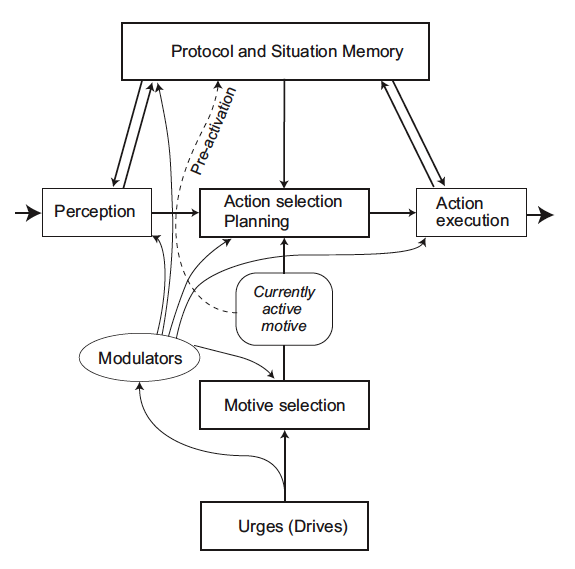
\includegraphics[width=11cm]{figures/Psi.png}
\caption{High-Level Architecture of the Psi Model}
\label{fig:Psi}
\end{figure}

\begin{itemize}
\item 能力需求(Competence):  智能体能有效实现某种强烈欲望的需求
\item 确定性需求(Certainty):智能体了解和熟悉环境的需求 
\end{itemize}

每种需求都有一定的偏好范围或目标范围,随着时间和环境(包括智能体自身)的不断变化,智能体的需求也在不断地变化。 当需求水平落在相应的目标范围时,
称作该需求被满足,否则需求不被满足。我们可以将智能体视为一个目标驱动的系统,其主要任务就是尽可能让所有这些需求都被满足。而当某一需求不被满足时,智能体会有一种试图将该需求水平恢复到偏好范围内的愿望,这种愿望便构成了{\bf 动机(Urge)}。


另外还有一种{\bf 愉悦感(Pleasure)}(和其反义的"不悦感")的原始概念,人们认为这种情绪与复杂的"幸福感"不同。愉悦感被解读成与愿望有关:当愿望(至少部分上)被满足,愉悦感便会由此而生;而当愿望愈趋强烈,不悦感则会由此产生。满足愿望的程度未必要被即刻定义;例如来说,它可被定义为一种需求对近期以来的目标范围随时间衰减的近似加权平均值。

因此,若智能体感到枯燥无趣,当受到大量新鲜感的刺激,它就会体验到某种愉悦感。若智能体感到枯燥无趣,而又更极端地受到单调的刺激,它就会体验到某种不悦感。

要注意的是,根据这相对简单的方法,任何幅度降低了不满感都会造成某种愉悦感;但若一切总是持续在其可接受的范围进行,就不会出现任何愉悦感。这看似有点违反直觉,但必须了解,这些简单的"愉悦感"与"不悦感"并不会完全掌握与这些字词相关的自然语言概念。此处使用的自然语言术语仅作为启发法传达涉及程序的一般特性。这些都是非常低水平的程序,在人类经验的相似情况远低于意识水平。
每个需求都有许多参数。如 Psi 模型所设,其中可调整的重要需求参数有:

\begin{itemize}
\item 权重:在特定时间点,相对于其他需求,该需求如何被加权
\item  增益:决定源自实现需求所得到的满足感多寡的定标因素
\item  损失:决定源自未实现需求所得到的未足之感多寡的定标因素
\item  衰减:基本上是被给定的愿望随着一段时间的增加率。

\end{itemize}

在此模型中,为刺激的缺乏使愿望随着时间增加。本人不确定这个模型是否与一般认知模型一样切实,但针对能确保某智能体持续在运作,这会是可行的短期机制。对应多种需求来调整增益、损失和衰竭等参数,便是变换智能体"个性"的一种方式。

接下来,{\bf 目标}被视为系统在未来某时间点致力成真的一种表达;而{\bf 动机}为一组 $(愿望, 目标)$配对,由一目标组成,该目标的满足感被预测隐含了某些愿望的满足感。事实上,愿望可被视为顶层目标(在 OpenCog 中有时又被称作 ”Ubergoals”),而智能体的其他目标则为子目标。"意图"也被视为综合体:在特定时间点的意图是由积极动机所构成,配合它们的相关目标、行为程序等。

在 Psi 模型中,智能体随时都有"主导动机";对 CogDial 的早期版本而言,虽然也是可行的假设,但大体上似乎是过度限制的假设,比起相似人类或其他高级人工智能系统,此假设或许更适合用在较单纯的模拟动物上。大致上可想成不同动机具有不同权重,而这些权重指出追求上所要耗费的资源量。

Psi 模型的基本行动逻辑是通过"三元祖"执行,非常类似 OpenCog 中的三元组$\textit{Context} \land \textit{Procedure} \rightarrow \textit{Goal}$ 。然而,有个重要角色是由四个调制因子扮演,其控制观感、认知和行动选择的程序如何在一特定时间受到规范:

\begin{itemize}
\item  活化度,决定智能体相对认知、反思活动,侧重于快速、密集活动的程度 
\item 分辨程度, 决定系统对于尝试解读世界的精准度 
\item 确定性,决定系统尝试达到确实、特定知识的努力程度 
\item 选择门槛,决定系统对改变其选择侧重的目标的意愿程度
\end{itemize}

这些调节因子在非常抽象的层次上表现出系统情绪和认知状态的特性;它们本质上并不是情绪,但它们对智能体的情绪有相当大的影响。它们预期的互动如图表\ref{fig:mod}所描述。


\begin{figure}[htb]
\centering
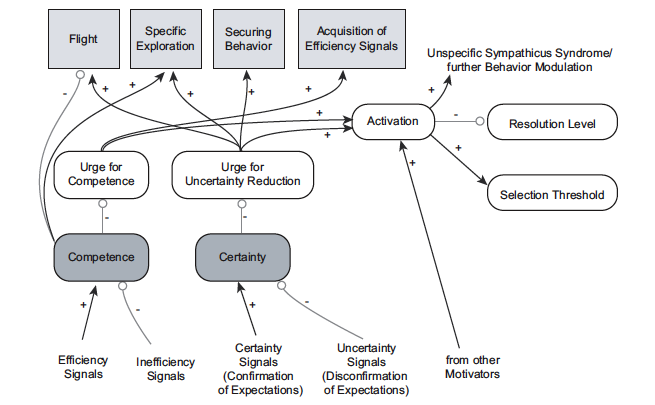
\includegraphics[width=12cm]{figures/PsiModulators.png}
\caption{Psi 调节因子之间的主要相互关系}
\label{fig:Mod}
\end{figure}

Psi 利用三个网络中安排的 Quad 储存知识,在概念上类似 Albus 的 4D/RCS 和 Arel 的 DeSTIN 结构:

\begin{itemize}

\item 储存陈述性知识的传感器网络:将图像、物体、事件呈现为分层结构的规划器 
\item 运动网络,通过阶层行为程序容纳过程知识
\item 处理需求的动机网络

\end{itemize}

Psi 模型的感知是根据 “HyPercept” 基于假设的感知的机制,其试图预测待理解的为何,并利用感知和记忆尝试验证这些预测。此外,根据对现实的探索和呈现之间的"Neisser知觉环",HyPercept 密切地联结外在世界的动作。感知上获得的信息会被转换为能够引导行为的规划器,再实施这些规划器(有时会显著影响世界),在进入用来引导进一步感知的程序。我们将不会利用 Psi 的这个层面,因 OpenCog 处理感知的方式不大相同。 
Psi 模型的动作选择是根据所谓的"三元组"运行,每个的组成是由

\begin{itemize}
\item 侦感器规划器(前置条件、"条件规划器";如 OpenCog 中的"语境")
\item 随后行动规划器(行动、效应器;如 OpenCog 中的"程序") 
\item 最终侦感器规划器(后置条件、预期;如 OpenCog 的谓语或目标)
\end{itemize}

区分这些三元组与用于 SOAR 和 ACT-R 中典型生产规则的不同之处,在于三元组可能不完整(三要素之中可能会缺少其中几个)且不确定。然而,在这三元组和 OpenCog 的概念/程序/目标三元组之间,似乎没有根本上的差异;MicroPsi 和 OpenCog 在此层面的差异,在于用于图解的基本知识呈现,以及用来表达含意的概率逻辑。
解出规划器待执行、以达到当前情境所选的目标,会在 Psi 模型中运用一种名叫"Rasmussen 阶梯理论"(以丹麦心理学家 Jens Rasmussen 之名命名)的程序结合来完成。Rasmussen 阶梯理论说明动作的组织,是这三种行为阶段的动作;其中有以技能为基础的行为、以规则为基础的行为和以知识为基础的行为:

\begin{itemize}
\item 若被给予的任务相当于训练过的例行程序,则会活化自动行为或技能;一般而言可不经由意识注意或慎重控制来执行。 
\item 若尚无自动行为,行动步骤可能会出自规则;在可采用一组已知策略之前,必须先对情况做分析,使策略适合用于情况。 
\item 若没有适用的已知策略,在这些情况下,必须先找出合并现有操作指令(运算元)到达成所设目标的方法。此阶段通常要求行为的重新构成,也就是规划的程序。
用于 Psi 和 MicroPsi 执行的规划算法是个相当简单的爬山法规划器。虽有人假设,针对高级智能也许会需要较复杂的规划器;但部分 Psi 模型的假设,是建立于一旦有机体具有正确的知觉表征和目标,大多数对该有机体进行实际规划所要做的,就相当简单。
\end{itemize}


在我们现使用的 CogDial 系统,如以下将说明的,为相应 Psi 模型中提及之前两种动作的认知规划器。某些感知规划器包含纯反射、自发行为(例如对"你好吗"的问题回答"我很好");其他则存有需要大量推理的行为。然而,目前 CogDial 的版本尚无法处理已知策略不适用的情况。大致上,OpenCog 确定会支持这种弹性情况,但我们仍在努力研究出有效运作于此对话语境中的更多基本行为。这是 CogDial 方法和纯发展性学习方法(这在 OpenCog 结构中也可能采取)之间的差异性;在效法人类幼童的认知和语言发展的发展性学习方法中,该基础在于处理已知策略不适用的情况,以及在此等情况下学习策略(虽有出生即具有相当高水平学习策略的论证,以及对多种有益于对话的行为之成见,但幼童并非一出生就具有任何处理对话情况的策略)。

%%%%%%%%%%%%%%%%%%%%%%%%%%%%%%%%
\section{Psi 模型中的情感与个性}{Emotion and Personality in the Psi Model}
%%%%%%%%%%%%%%%%%%%%%%%%%%%%%%%%

情感是人类心理学和人机交互的重要层面。若对话系统能够做到情感的自然互动,对人类谈话对象而言,自动化自然语言对话将更加受人注目且令人满意。要将情感自然度注入到对话中,Psi 模型会是合适的方法,因其含有栩栩如生的人类情感模型 。
Psi 中的情感被视为复杂的系统响应模式,而不是清楚构建出的实体。情感是响应某特定愿望所唤起的心理实体。在 Bach 的论文 \cite{Bach2012} "涌现的情感"(”Emergent Emotions”) 中,他将特定的情感与基本的调制器值建立关连,例如:

\begin{itemize}
\item 愤怒(Anger):负价、高激发性、低决断水平、选择阈值高
\item 伤心(Sadness):负价、低激发性、高决断水平、低防御度、低意图性 
\item 喜悦(Joy):正价、高激发性、低决断水平
\item 福佑(Bliss):正价、低激发性、高决断水平
\item 沮丧(Frustration):负价、中等激发性、低决断水平、选择阈值低(此为近期才加入到本文的研究中,而前面的项目则是出自前文提及之 Bach 的论文)
\end{itemize}

这类关系在概念上的性质或许值得强调。我们并不是在试图将人类的情感以任何意义上"降低"为调制器值的结合。确切的说,我们认为如"愤怒"、"喜悦"等情绪字词,都是对复杂的人类心理动力极原始的叙述。通过适当地合并调节器的值,我们就可经由许多情感字词所示的指出系统动力空间惯常上稍接近的区域。当然人脑/人体的动力系统含有许多未在 Psi 中建模的复杂参数,我们并不尝试做出精准无误的神经生理情感模型。
个性 – 在对话语境中也是个有趣的话题。若想创建显示多种个性特质的对话系统,可能要以密切相关的方式来处理。经典的人格"五大因素"模型,是使用五种因素来解释人类个性的变异:

\begin{itemize}
\item 直率性(openness)
\item 尽责性( conscientiousness)
\item 外向性 (extraversion)
\item 亲和性(agreeableness)
\item 情绪不稳定性(neuroticism)
\end{itemize}

"涌现的情绪"(”Emergent Emotions”)文中论证,这些至少可从增益、衰减和损失参数的角度粗略地解释归属感、竞争、确定性和美感等需求。 
基于这点,可根据多种需求的参数来撰写计算所设人物五大因素每项估计值的程式码。或者也可逆转数学,写出简单的等式,其中含有

\begin{itemize}
\item 输入:针对五大人格因素的量性度量,与特定人物相联系 
\item 输出:针对归属感、竞争、确定性和美感等需求的具体增益、损失和衰减参数值,意图相应于人格五大因素的指定的值
\end{itemize}

通过对每项人格五大因素(例如个性被指定为五维向量)从范围 [0,1] 指定一个数字,即可在建构档案中指定一人物的个性。当然与人类个性的错综复杂相比,这显然较粗糙;但针对适合的特殊应用情况,配合提供的对话系统个性内容,在合理程度上这会是很务实的工具。

%%%%%%%%%%%%%%%%%%%%%%%%%%%%%%%%%%%%%%%%%%%%%%%%%%%%%%%%%%%%%%%
\section{本章小结}{Summary of Accomplishments and Future Work}
%%%%%%%%%%%%%%%%%%%%%%%%%%%%%%%%%%%%%%%%%%%%%%%%%%%%%%%%%%%%%%%

XXX
%%%%%%%%%%%%%%%%%%%%%%%%%%%%%%%%%%%%%%%%%%%%%%%%%
